\documentclass{article}

\usepackage{amsmath,amssymb}
\usepackage{tikz}
\usepackage{pgfplots}
\usepackage{xcolor}
\usepackage[left=2.1cm,right=3.1cm,bottom=3cm,footskip=0.75cm,headsep=0.5cm]{geometry}
\usepackage{enumerate}
\usepackage{enumitem}
\usepackage{marvosym}
\usepackage{tabularx}
\usepackage{parskip}

\usepackage{listings}
\definecolor{lightlightgray}{rgb}{0.95,0.95,0.95}
\definecolor{lila}{rgb}{0.8,0,0.8}
\definecolor{mygray}{rgb}{0.5,0.5,0.5}
\definecolor{mygreen}{rgb}{0,0.8,0.26}
\lstdefinestyle{R} {language=R,morekeywords={confint,head,fitdist,ks,test}}
\lstset{language=R,
	basicstyle=\ttfamily,
	keywordstyle=\color{lila},
	commentstyle=\color{lightgray},
	stringstyle=\color{mygreen}\ttfamily,
	backgroundcolor=\color{white},
	showstringspaces=false,
	numbers=left,
	numbersep=10pt,
	numberstyle=\color{mygray}\ttfamily,
	identifierstyle=\color{blue},
	xleftmargin=.1\textwidth, 
	%xrightmargin=.1\textwidth,
	escapechar=§,
}
\usepackage[colorlinks = true, linkcolor = blue, urlcolor  = blue, citecolor = blue, anchorcolor = blue]{hyperref}

\usepackage[utf8]{inputenc}

\renewcommand*{\arraystretch}{1.4}

\newcolumntype{L}[1]{>{\raggedright\arraybackslash}p{#1}}
\newcolumntype{R}[1]{>{\raggedleft\arraybackslash}p{#1}}
\newcolumntype{C}[1]{>{\centering\let\newline\\\arraybackslash\hspace{0pt}}m{#1}}

\newcommand{\E}{\mathbb{E}}
\DeclareMathOperator{\Var}{Var}
\DeclareMathOperator{\CDF}{CDF}

\title{\textbf{Wie funktioniert Maximum-Likelihood-Schätzung?}}
\author{\textsc{Henry Haustein}}
\date{}

\begin{document}
	\maketitle
	
	\section*{Vom Speziellen...}
	Aus einem Zufallszahlengenerator $X$ erhalten wir die folgenden 5 Zufallszahlen: 3, 4, 4, 4, 5. Wir wissen außerdem, dass die Zufallszahlen exponentialverteilt und unabhängig sind, aber wir kennen den Parameter der Verteilung nicht. Wie können wir diesen bestimmen?
	
	Schauen wir uns zuerst an, wie \textit{wahrscheinlich}\footnote{Die Exponentialverteilung ist eine stetige Verteilung, das heißt die Wahrscheinlichkeit, eine bestimmte Zahl zu erhalten, ist per Definition 0. Statt von Wahrscheinlichkeiten wäre es besser von Plausibiltäten zu sprechen, aber das macht den Text weniger gut lesbar.} es ist, eine der obigen Zufallszahlen erhalten zu haben, abhängig vom Parameter der Exponentialverteilung
	\begin{align}
		\mathbb{P}(X=3) &= \lambda\cdot \exp(-3\cdot \lambda) \notag \\
		\mathbb{P}(X=4) &= \lambda\cdot \exp(-4\cdot \lambda) \notag \\
		\mathbb{P}(X=4) &= \lambda\cdot \exp(-4\cdot \lambda) \notag \\
		\mathbb{P}(X=4) &= \lambda\cdot \exp(-4\cdot \lambda) \notag \\
		\mathbb{P}(X=5) &= \lambda\cdot \exp(-5\cdot \lambda) \notag
	\end{align}
	Wir sollten also den Parameter $\lambda$ so wählen, dass die \textit{Wahrscheinlichkeiten} für alle diese Ereignisse möglichst groß werden.
	
	Wir könnten uns anschauen, wie \textit{wahrscheinlich} es ist, dass wir alle Zufallszahlen sehen: Dazu nutzen wir die Eigenschaft, dass die Zufallszahlen unabhängig sind und erinnern uns an
	\begin{align}
		\mathbb{P}(A\text{ und } B) = \mathbb{P}(A)\cdot \mathbb{P}(B) \notag
	\end{align}
	Wir erweitern diese Idee auf unsere 5 Zufallszahlen und erhalten:
	\begin{align}
		\mathbb{P}(\text{alle obigen Zufallszahlen gesehen}) = \mathbb{P}(X=3) \cdot \mathbb{P}(X=4)\cdot\mathbb{P}(X=4)\cdot\mathbb{P}(X=4)\cdot\mathbb{P}(X=5) \notag
	\end{align}
	Wir nennen diesen Term die Likelihood-Funktion $L(\lambda)$. Diese gibt an, wie \textit{wahrscheinlich} (bzw. plausibel) es ist, dass wir die obigen Zufallszahlen bekommen haben, in Abhängigkeit des Parameters $\lambda$.
	\begin{align}
		L(\lambda) &= \Big(\lambda\cdot\exp(-3\lambda)\Big)\cdot \Big(\lambda\cdot\exp(-4\lambda)\Big)\cdot \Big(\lambda\cdot\exp(-4\lambda)\Big)\cdot \Big(\lambda\cdot\exp(-4\lambda)\Big)\cdot \Big(\lambda\cdot\exp(-5\lambda)\Big) \notag \\
		&= \lambda^5 \cdot \exp(-3\lambda)\exp(-4\lambda)\exp(-4\lambda)\exp(-4\lambda)\exp(-5\lambda) \notag \\
		&= \lambda^5\cdot\exp(-3\lambda + -4\lambda + -4\lambda + -4\lambda + -5\lambda) \notag \\
		&= \lambda^5\cdot\exp(-20\lambda) \notag
	\end{align}
	Wir wollen die Likelihood-Funktion maximieren, dafür könnten wir $L(\lambda)$ nach $\lambda$ ableiten und nullsetzen. Aber für einige Verteilungen ist das ziemlich aufwendig, da wir die Produktregel für Ableitungen benutzen müssten. Wir greifen deswegen auf einen kleinen Trick zurück und bilden $l(\lambda) = \log(L(\lambda))$. Diese Funktion heißt log-Likelihood-Funktion und hat die Eigenschaft, dass das Maximum dieser genau beim selben $\lambda$ wie bei $L(\lambda)$ ist.
	\begin{center}
		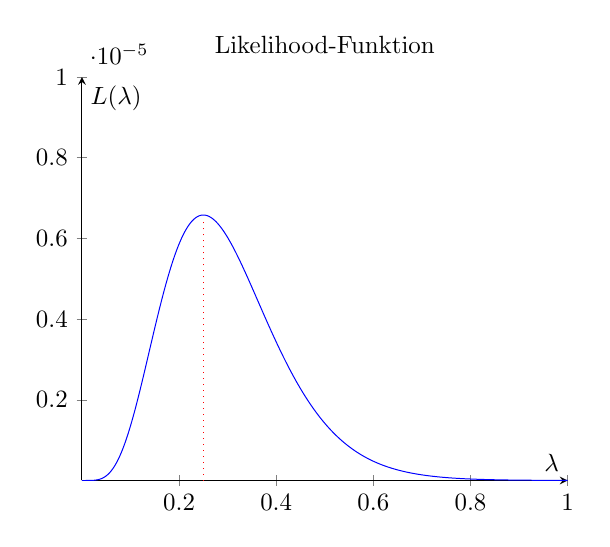
\begin{tikzpicture}[scale=0.9]
			\begin{axis}[
				xmin=0, xmax=1, xlabel=$\lambda$,
				ymin=0, ymax=0.00001, ylabel=$L(\lambda)$,
				title={Likelihood-Funktion},
				samples=400,
				axis x line=middle,
				axis y line=middle,
				domain=0:1,
				]
				\addplot[mark=none,smooth,blue] {x*x*x*x*x*exp(-20*x)};
				\draw[red, dotted] (axis cs: 0.25, 0) -- (axis cs: 0.25, 0.0000065);
				
			\end{axis}
		\end{tikzpicture}
		\begin{tikzpicture}[scale=0.9]
			\begin{axis}[
				xmin=0, xmax=1, xlabel=$\lambda$,
				ymin=-25, ymax=0, ylabel=$l(\lambda)$,
				title={log-Likelihood-Funktion},
				samples=400,
				axis x line=middle,
				axis y line=middle,
				domain=0:1,
				restrict y to domain=-25:0
				]
				\addplot[mark=none,smooth,blue] {5*ln(x)-20*x)};
				\draw[red, dotted] (axis cs: 0.25, 0) -- (axis cs: 0.25, -11.931);
				
			\end{axis}
		\end{tikzpicture}
	\end{center}
	Die log-Likelihood-Funktion sieht so aus:
	\begin{align}
		l(\lambda) &= \log\Big(\lambda^5\cdot \exp(-20\lambda)\Big) \notag \\
		&= \log(\lambda^5) + \log(\exp(-20\lambda)) \notag \\
		&= 5\cdot\log(\lambda) - 20\lambda \notag
	\end{align}
	Diese Funktion ist viel leichter abzuleiten, weil der Logarithmus alle Produkte in Summen verwandelt.
	
	Maximieren von $l(\lambda)$ liefert:
	\begin{align}
		\frac{\partial l}{\partial\lambda} &= 5\cdot\frac{1}{\lambda} - 20 \overset{!}{=} 0 \notag \\
		20 &= \frac{5}{\lambda} \notag \\
		\lambda &= \frac{5}{20} = \frac{1}{4} \notag
	\end{align}
	Damit haben wir eine Schätzung für den Parameter $\lambda$ gefunden. Man sollte aber noch bedenken, dass dies der plausibelste Parameter ist - wir wissen nicht mit Sicherheit, welchen wahren Wert der Parameter in unserem Zufallsgenerator hat.
	
	\section*{... ins Allgemeine}
	
	Wir betrachten nun den Fall, dass wir nicht mehr nur 5 Zufallszahlen, sondern $n$ Zufallszahlen $x_1, ..., x_n$ haben. Die \textit{Wahrscheinlichkeit}, dass unser Zufallszahlengenerator nun eine dieser Zahlen ausgibt, ist
	\begin{align}
		\mathbb{P}(X=x_1) &= \lambda\cdot\exp(-\lambda x_1) \notag \\
		\mathbb{P}(X=x_2) &= \lambda\cdot\exp(-\lambda x_2) \notag \\
		&\vdots \notag \\
		\mathbb{P}(X=x_n) &= \lambda\cdot\exp(-\lambda x_n) \notag
	\end{align}
	Die \textit{Wahrscheinlichkeit}, dass wir alle $n$ Zufallszahlen sehen, ist
	\begin{align}
		\mathbb{P}(\text{alle $n$ Zufallszahlen gesehen}) &= \mathbb{P}(X=x_1) \cdot \mathbb{P}(X=x_2)\cdot\dots\cdot \mathbb{P}(X=x_n) \notag \\
		&= \prod_{i=1}^{n} \mathbb{P}(X=x_i) \notag
	\end{align}
	Das ist die Likelihood-Funktion $L(\lambda)$; ausgeschrieben ist sie
	\begin{align}
		L(\lambda) &= \prod_{i=1}^n \mathbb{P}(X=x_i) \notag \\
		&= \prod_{i=1}^n \lambda\cdot\exp(-\lambda x_i) \notag \\
		&= \lambda^n \cdot\prod_{i=1}^n \exp(-\lambda x_i) \notag \\
		&= \lambda^n \cdot\exp\left(\sum_{i=1}^{n} -\lambda x_i\right) \notag \\
		&= \lambda^n\cdot\exp\left(-\lambda\sum_{i=1}^n x_i\right) \notag
	\end{align}
	Diese Funktion wollen wir wieder maximieren, aber die Ableitung erweist sich hier als schwierig. Deswegen nutzen wir den Trick mit dem logarithmieren und erhalten die log-Likelihood-Funktion $l(\lambda)$:
	\begin{align}
		\l(\lambda) &= \log(L(\lambda)) \notag \\
		&= \log\left(\lambda^n\cdot\exp\left(-\lambda\sum_{i=1}^n x_i\right)\right) \notag \\
		&= \log\left(\lambda^n\right) + \log\left(\exp\left(-\lambda\sum_{i=1}^n x_i\right)\right) \notag \\
		&= n\log(\lambda) - \lambda\sum_{i=1}^{n} x_i \notag
	\end{align}
	Ableiten und nullsetzen liefert
	\begin{align}
		\frac{\partial l}{\partial \lambda} &= \frac{n}{\lambda} - \sum_{i=1}^n x_i \overset{!}{=} 0 \notag \\
		\sum_{i=1}^n x_i &= \frac{n}{\lambda} \notag \\
		\lambda &= \frac{n}{\sum_{i=1}^n x_i} = \frac{1}{\bar{x}} \notag
	\end{align}
	Damit haben wir den allgemeinen Schätzer der Exponentialverteilung gefunden.
\end{document}